\documentclass{standalone}
\usepackage{tikz}
\usetikzlibrary{patterns, positioning}
\usepackage[sfdefault]{ClearSans} %% option 'sfdefault' activates Clear Sans as the default text font
\usepackage[T1]{fontenc}

\begin{document}
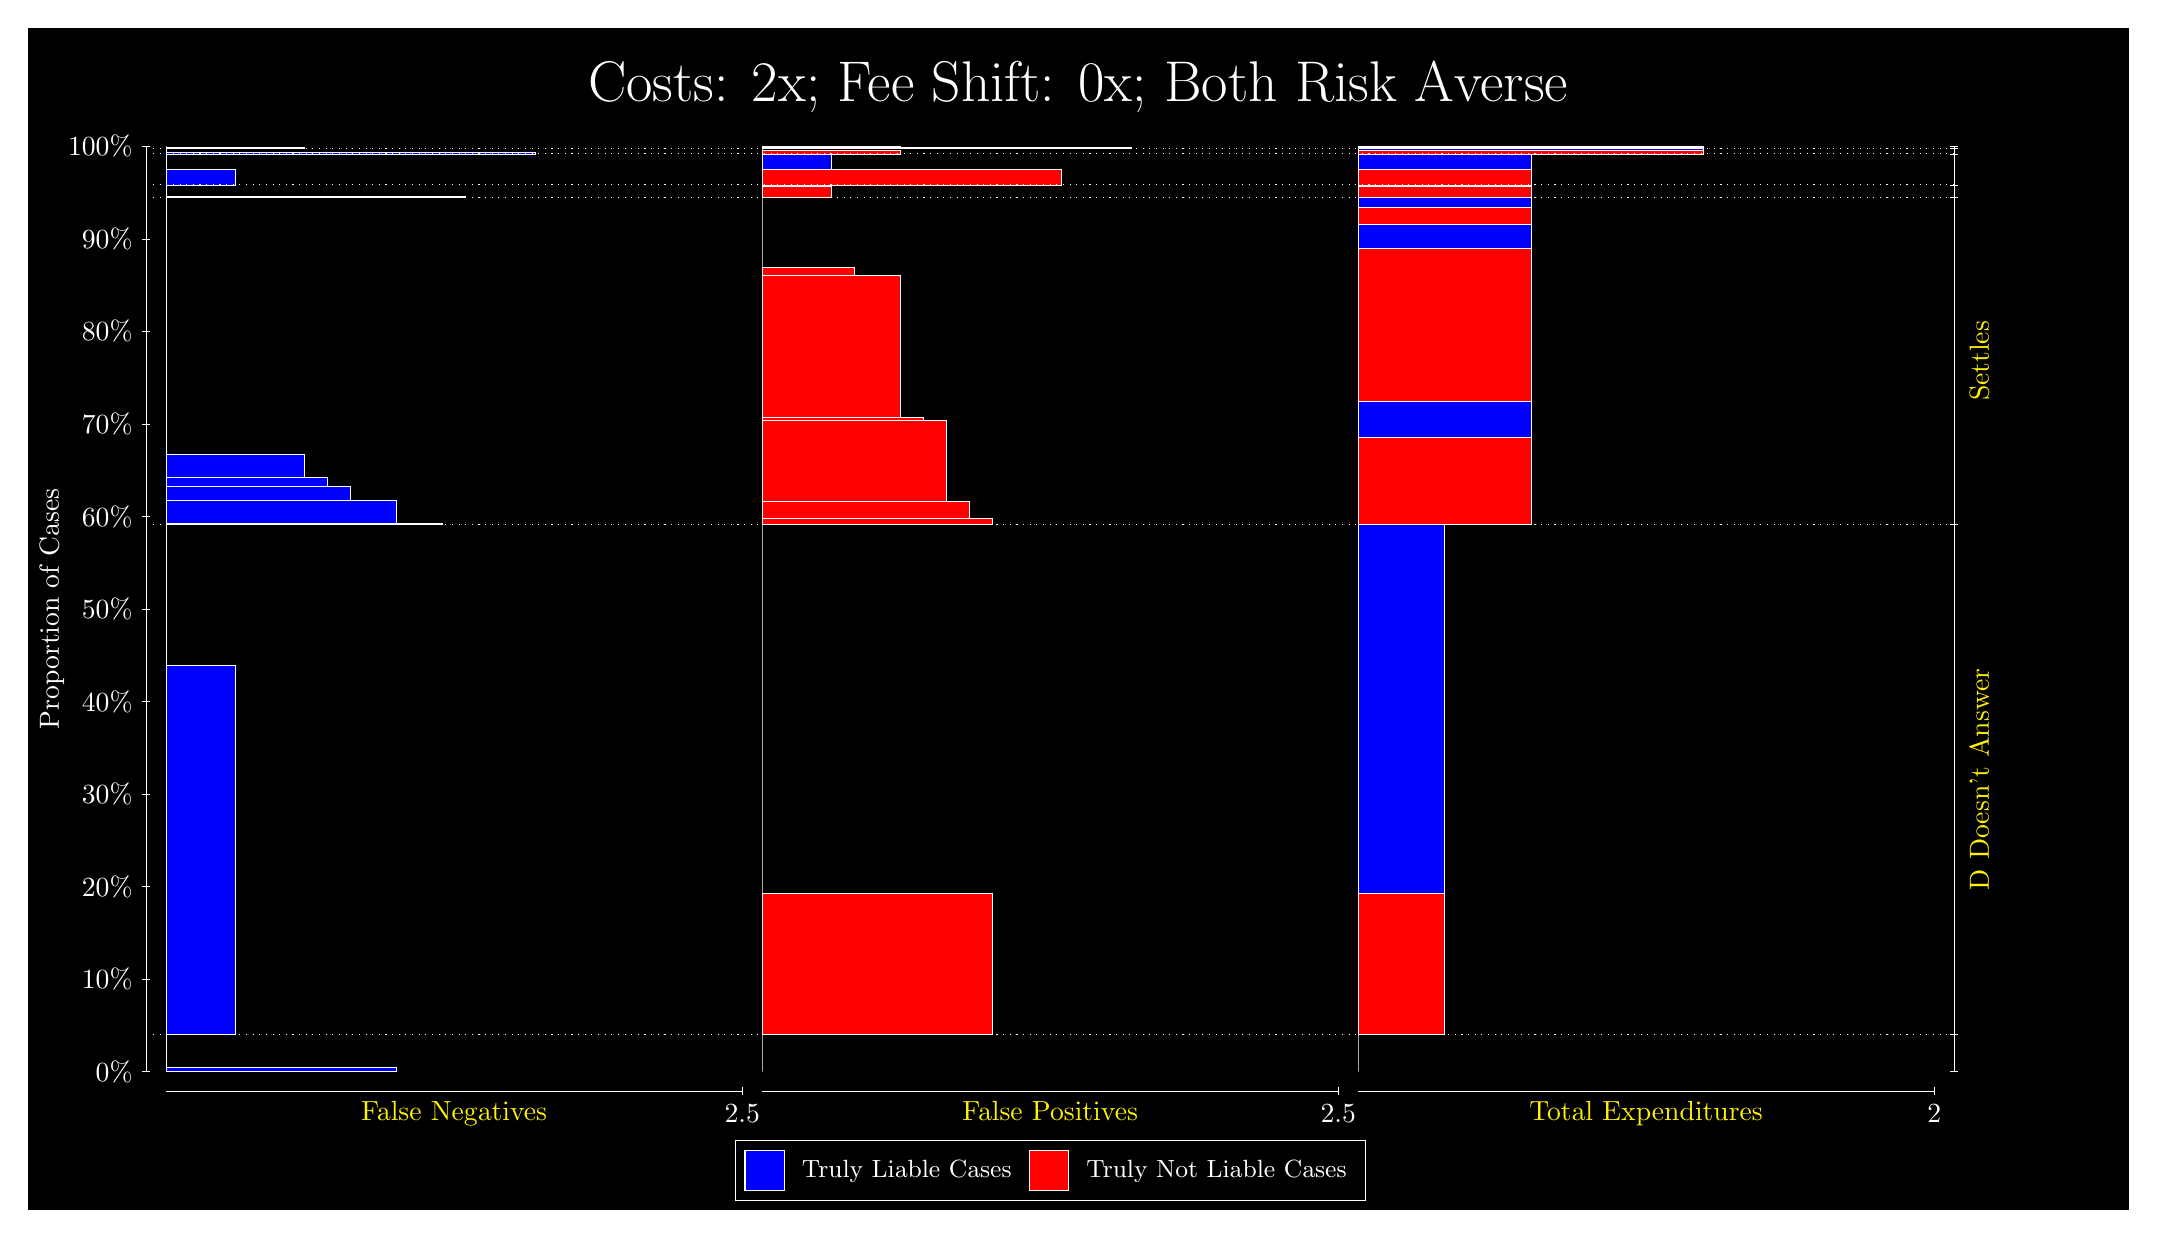
\begin{tikzpicture}
\draw[fill=black] (0,0) rectangle (26.667,15);
\draw[text=white] (0,13.5) rectangle (26.667,15) node[midway] {\huge Costs: 2x; Fee Shift: 0x; Both Risk Averse};
\draw[white, very thin] (1.5,1.75) -- (1.5,13.5);
\node[rotate=90, text=white, anchor=center] at (0.3, 7.625) {Proportion of Cases};
\draw[white, very thin] (1.45,1.75) -- (1.55,1.75);
\node[text=white, anchor=east] at (1.45, 1.75) {0\%};
\draw[white, very thin] (1.45,2.925) -- (1.55,2.925);
\node[text=white, anchor=east] at (1.45, 2.925) {10\%};
\draw[white, very thin] (1.45,4.1) -- (1.55,4.1);
\node[text=white, anchor=east] at (1.45, 4.1) {20\%};
\draw[white, very thin] (1.45,5.275) -- (1.55,5.275);
\node[text=white, anchor=east] at (1.45, 5.275) {30\%};
\draw[white, very thin] (1.45,6.45) -- (1.55,6.45);
\node[text=white, anchor=east] at (1.45, 6.45) {40\%};
\draw[white, very thin] (1.45,7.625) -- (1.55,7.625);
\node[text=white, anchor=east] at (1.45, 7.625) {50\%};
\draw[white, very thin] (1.45,8.8) -- (1.55,8.8);
\node[text=white, anchor=east] at (1.45, 8.8) {60\%};
\draw[white, very thin] (1.45,9.975) -- (1.55,9.975);
\node[text=white, anchor=east] at (1.45, 9.975) {70\%};
\draw[white, very thin] (1.45,11.15) -- (1.55,11.15);
\node[text=white, anchor=east] at (1.45, 11.15) {80\%};
\draw[white, very thin] (1.45,12.325) -- (1.55,12.325);
\node[text=white, anchor=east] at (1.45, 12.325) {90\%};
\draw[white, very thin] (1.45,13.5) -- (1.55,13.5);
\node[text=white, anchor=east] at (1.45, 13.5) {100\%};

\draw[white, very thin] (24.457,1.75) -- (24.457,13.5);
\draw[white, very thin] (24.407,1.75) -- (24.507,1.75);
\node[anchor=west] at (24.407, 1.75) {};
\draw[white, very thin] (24.407,2.2185) -- (24.507,2.2185);
\node[anchor=west] at (24.407, 2.2185) {};
\draw[white, very thin] (24.407,8.7025) -- (24.507,8.7025);
\node[anchor=west] at (24.407, 8.7025) {};
\draw[white, very thin] (24.407,12.848) -- (24.507,12.848);
\node[anchor=west] at (24.407, 12.848) {};
\draw[white, very thin] (24.407,13.011) -- (24.507,13.011);
\node[anchor=west] at (24.407, 13.011) {};
\draw[white, very thin] (24.407,13.404) -- (24.507,13.404);
\node[anchor=west] at (24.407, 13.404) {};
\draw[white, very thin] (24.407,13.47) -- (24.507,13.47);
\node[anchor=west] at (24.407, 13.47) {};
\draw[white, very thin] (24.407,13.5) -- (24.507,13.5);
\node[anchor=west] at (24.407, 13.5) {};

\draw[white, very thin, fill=blue] (1.75,1.75) rectangle (4.6775,1.7993);
\draw[white, very thin, fill=red] (1.75,1.7993) rectangle (1.75,2.2185);
\draw[white, very thin, fill=blue] (1.75,2.2185) rectangle (2.6283,6.9096);
\draw[white, very thin, fill=red] (1.75,6.9096) rectangle (1.75,8.7025);
\draw[white, very thin, fill=blue] (1.75,8.7025) rectangle (5.2631,8.719);
\draw[white, very thin, fill=blue] (1.75,8.719) rectangle (4.6775,8.999);
\draw[white, very thin, fill=blue] (1.75,8.999) rectangle (4.3848,9.0101);
\draw[white, very thin, fill=blue] (1.75,9.0101) rectangle (4.092,9.1818);
\draw[white, very thin, fill=blue] (1.75,9.1818) rectangle (3.7993,9.2996);
\draw[white, very thin, fill=blue] (1.75,9.2996) rectangle (3.5065,9.5913);
\draw[white, very thin, fill=red] (1.75,9.5913) rectangle (1.75,12.848);
\draw[white, very thin, fill=blue] (1.75,12.848) rectangle (5.5558,12.871);
\draw[white, very thin, fill=red] (1.75,12.871) rectangle (1.75,13.011);
\draw[white, very thin, fill=blue] (1.75,13.011) rectangle (2.6283,13.203);
\draw[white, very thin, fill=red] (1.75,13.203) rectangle (1.75,13.404);
\draw[white, very thin, fill=blue] (1.75,13.404) rectangle (6.4341,13.419);
\draw[white, very thin, fill=red] (1.75,13.419) rectangle (1.75,13.47);
\draw[white, very thin, fill=blue] (1.75,13.47) rectangle (3.5065,13.485);
\draw[white, very thin, fill=red] (1.75,13.485) rectangle (1.75,13.5);
\draw[white, very thin, fill=red] (9.3189,1.75) rectangle (9.3189,2.1692);
\draw[white, very thin, fill=blue] (9.3189,2.1692) rectangle (9.3189,2.2185);
\draw[white, very thin, fill=red] (9.3189,2.2185) rectangle (12.246,4.0113);
\draw[white, very thin, fill=blue] (9.3189,4.0113) rectangle (9.3189,8.7025);
\draw[white, very thin, fill=red] (9.3189,8.7025) rectangle (12.246,8.7738);
\draw[white, very thin, fill=red] (9.3189,8.7738) rectangle (11.954,8.9919);
\draw[white, very thin, fill=red] (9.3189,8.9919) rectangle (11.661,10.018);
\draw[white, very thin, fill=red] (9.3189,10.018) rectangle (11.368,10.059);
\draw[white, very thin, fill=red] (9.3189,10.059) rectangle (11.075,11.856);
\draw[white, very thin, fill=red] (9.3189,11.856) rectangle (10.49,11.959);
\draw[white, very thin, fill=blue] (9.3189,11.959) rectangle (9.3189,12.848);
\draw[white, very thin, fill=red] (9.3189,12.848) rectangle (10.197,12.987);
\draw[white, very thin, fill=blue] (9.3189,12.987) rectangle (9.3189,13.011);
\draw[white, very thin, fill=red] (9.3189,13.011) rectangle (13.125,13.212);
\draw[white, very thin, fill=blue] (9.3189,13.212) rectangle (10.197,13.404);
\draw[white, very thin, fill=red] (9.3189,13.404) rectangle (11.075,13.455);
\draw[white, very thin, fill=blue] (9.3189,13.455) rectangle (9.3189,13.47);
\draw[white, very thin, fill=red] (9.3189,13.47) rectangle (14.003,13.485);
\draw[white, very thin, fill=blue] (9.3189,13.485) rectangle (11.075,13.5);
\draw[white, very thin, fill=red] (16.888,1.75) rectangle (16.888,2.1692);
\draw[white, very thin, fill=blue] (16.888,2.1692) rectangle (16.888,2.2185);
\draw[white, very thin, fill=red] (16.888,2.2185) rectangle (17.986,4.0113);
\draw[white, very thin, fill=blue] (16.888,4.0113) rectangle (17.986,8.7025);
\draw[white, very thin, fill=red] (16.888,8.7025) rectangle (19.083,9.8002);
\draw[white, very thin, fill=blue] (16.888,9.8002) rectangle (19.083,10.264);
\draw[white, very thin, fill=red] (16.888,10.264) rectangle (19.083,12.204);
\draw[white, very thin, fill=blue] (16.888,12.204) rectangle (19.083,12.512);
\draw[white, very thin, fill=red] (16.888,12.512) rectangle (19.083,12.73);
\draw[white, very thin, fill=blue] (16.888,12.73) rectangle (19.083,12.848);
\draw[white, very thin, fill=red] (16.888,12.848) rectangle (19.083,12.987);
\draw[white, very thin, fill=blue] (16.888,12.987) rectangle (19.083,13.011);
\draw[white, very thin, fill=red] (16.888,13.011) rectangle (19.083,13.212);
\draw[white, very thin, fill=blue] (16.888,13.212) rectangle (19.083,13.404);
\draw[white, very thin, fill=red] (16.888,13.404) rectangle (21.279,13.455);
\draw[white, very thin, fill=blue] (16.888,13.455) rectangle (21.279,13.47);
\draw[white, very thin, fill=red] (16.888,13.47) rectangle (21.279,13.485);
\draw[white, very thin, fill=blue] (16.888,13.485) rectangle (21.279,13.5);
\draw[white, dotted] (1.5,2.2185) -- (24.457,2.2185);
\draw[white, dotted] (1.5,8.7025) -- (24.457,8.7025);
\draw[white, dotted] (1.5,12.848) -- (24.457,12.848);
\draw[white, dotted] (1.5,13.011) -- (24.457,13.011);
\draw[white, dotted] (1.5,13.404) -- (24.457,13.404);
\draw[white, dotted] (1.5,13.47) -- (24.457,13.47);
\draw[white, very thin] (1.75,1.5) -- (9.0689,1.5);
\node[text=yellow, anchor=north] at (5.4094, 1.5) {False Negatives};
\draw[white, very thin] (9.0689,1.45) -- (9.0689,1.55);
\node[text=white, anchor=north] at (9.0689, 1.45) {2.5};

\draw[white, very thin] (9.3189,1.5) -- (16.638,1.5);
\node[text=yellow, anchor=north] at (12.978, 1.5) {False Positives};
\draw[white, very thin] (16.638,1.45) -- (16.638,1.55);
\node[text=white, anchor=north] at (16.638, 1.45) {2.5};

\draw[white, very thin] (16.888,1.5) -- (24.207,1.5);
\node[text=yellow, anchor=north] at (20.547, 1.5) {Total Expenditures};
\draw[white, very thin] (24.207,1.45) -- (24.207,1.55);
\node[text=white, anchor=north] at (24.207, 1.45) {2};


\node[text=yellow, centered, rotate=90] at (24.777, 5.4605) {D Doesn't Answer};
\node[text=yellow, centered, rotate=90] at (24.777, 10.775) {Settles};





\draw (12.978300999999998,1.5) node[draw=none] (baseCoordinate) {};
\begin{scope}[align=center]
        \matrix[scale=0.5, draw=white, below=0.5cm of baseCoordinate, nodes={draw}, column sep=0.1cm]{
            \node[rectangle, draw, minimum width=0.5cm, minimum height=0.5cm, fill=blue] {}; &
            \node[draw=none, font=\small, text=white] (B) {Truly Liable Cases}; &
            \node[rectangle, draw, minimum width=0.5cm, minimum height=0.5cm, fill=red] {}; &
            \node[draw=none, font=\small, text=white] (B) {Truly Not Liable Cases}; \\
            };
\end{scope}

\end{tikzpicture}
\end{document}